%-----------------------------------------------------------------------------
%
%               Template for sigplanconf LaTeX Class
%
% Name:         sigplanconf-template.tex
%
% Purpose:      A template for sigplanconf.cls, which is a LaTeX 2e class
%               file for SIGPLAN conference proceedings.
%
% Author:       Paul C. Anagnostopoulos
%               Windfall Software
%               978 371-2316
%               paul@windfall.com
%
% Created:      15 February 2005
%
%-----------------------------------------------------------------------------


\documentclass[10pt, preprint]{sigplanconf}

% The following \documentclass options may be useful:
%
% 10pt          To set in 10-point type instead of 9-point.
% 11pt          To set in 11-point type instead of 9-point.
% authoryear    To obtain author/year citation style instead of numeric.

\usepackage{amsmath}
\usepackage{graphicx}
\usepackage{subfigure}
\usepackage{multirow}
\usepackage{rotating}
\usepackage{array}
\usepackage{algorithmic}
\usepackage{algorithm}
\usepackage{textcomp}
\usepackage{listings}
\usepackage{hyperref}
%\usepackage{cite} %after hyperref

\begin{document}

\conferenceinfo{WXYZ '05}{date, City.} 
\copyrightyear{2011} 
\copyrightdata{[to be supplied]} 

\titlebanner{preprint}        % These are ignored unless
\preprintfooter{Naming Anonymous JavaScript Functions}   % 'preprint' option specified.

%\title{Better JavaScript Runtime Understanding by Automated Function Name Extraction}
%\title{JavaScript Lost Names, Is There Any Solution?}
%\title{JavaScript Lost Names, Any Amendment?}
%\title{Fixing Lost JavaScript Function Names in Debuggers}
\title{Naming Anonymous JavaScript Functions}
%\subtitle{Subtitle Text, if any}

\authorinfo{Salman Mirghasemi}
           {\'Ecole Polytechnique F\'ed\'erale de Lausanne(EPFL)}
           {salman.mirghasemi@epfl.ch}
\authorinfo{John J. Barton}
           {IBM Research - Almaden}
           {bartonjj@us.ibm.com} 
\authorinfo{Claude Petitpierre}
           {\'Ecole Polytechnique F\'ed\'erale de Lausanne(EPFL)}
           {claude.petitpierre@epfl.ch}

\maketitle

\begin{abstract}
JavaScript developers create and call functions; they use functions to construct objects. JavaScript development tools need to report to developers about those functions and constructors, for example in debugger call-stacks and object representations. However, developers need not specify names for functions.  
 Based on our analysis of ten large, widely used JavaScript projects, less than 7\% of JavaScript functions are named by developers. 
By studying examples from these JavaScript projects, we propose Static Function-Object Consumption, a principled, automated approach based on local source code analysis for naming nameless JavaScript functions.  We applied our approach to these same JavaScript projects and the results are very promising.
\end{abstract}

\category{D.2.5}{Testing and Debugging}{Debugging aids}
\category{D.2.6}{Programming Environments}{Integrated environments}

\terms
Algorithms, Human Factors, Languages

\keywords
JavaScript, Anonymous Function Name, Debugger

\section{Introduction}
The unique and important role of JavaScript in web programming is undeniable. Along with the wave of ``Web 2.0", JavaScript has become the inevitable part of almost every modern web site. This language is used by all of the web's 100 most popular sites\footnote[1]{http://www.alexa.com}. It is very likely that JavaScript keeps this crucial role for the next few years or even the next decade. Along with the growth of demands for more comprehensive user interfaces, the size and the complexity of web applications is increasing. Moreover, JavaScript is also becoming a general purpose computing platform with office applications \cite{JSOffice, JSOffice2}, browsers \cite{FAO, GCE} and development environments \cite{Ingalls} being developed in JavaScript \cite{Richards}. There are also proposals for employing JavaScript in server-side applications \cite{SSJSR, CJS}.

To cope with these large and sophisticated systems, JavaScript developers turn to better development tools. These tools analyze then represent the program in ways that the developer might only be able to imagine through substantial time-consuming reading of source code.  One prime example is a runtime debugger: the developer can halt a running program and examine the program state and execution call stack. 

All of these tools need to express program artifacts in a compact way the developer can understand.  For example, the debugger needs to present the execution call stack so the developer can understand which functions are currently active.  Obviously a particularly good compact representation would be a name given by the developer in the source code. However, the JavaScript language itself does not require names for many program artifacts and -- as we shall see -- nameless or anonymous artifacts are more common than named ones. Anonymous artifacts prevent tools from communicating effectively with developers.

Among program artifacts, functions are central to program comprehension in JavaScript. In addition to their role in the execution stack, they are first-class objects that are used for different purposes by developers; they may be used as an object constructor, a closure scope (module) or even  passed as an argument in a function call. However, functions can be defined and created without a name or identifier.  

In this paper, we analyze ten large, well-known projects. We show that within these projects less than 7\% of the function bodies are named. 
We analyze the syntactic constructs that function bodies appear in and rationalize how developers think about the bodies in relation to the structure of the code.
We propose an automated approach based on extracted data from the source code for naming JavaScript functions. The candidate function names can be used in debuggers for more descriptive object summaries and call-stack view, or in integration with proposed JavaScript typing systems for providing modern editing features in development environments. 


%In this paper, we analyze function creation and consumption in ten famous project. We propose an automated approach based on extracted data from the source code for naming JavaScript functions. The candidate function names can be used in debuggers for more descriptive object summaries and call-stack view, or in integration with proposed JavaScript typing systems for providing modern editing features in development environments. 
%The function name is necessary for referring and recalling the function's functionality, but only a small proportion (less than 7\%) of JavaScript functions are named.


\begin{table}

\centering
\scalebox{0.8}{
  \begin{tabular}{ | l | l | l | l | l |}
  \hline
   Project & Description & Total & Named \\ 
  \hline 
   Closure & Google Web Library & 9195 & 208(2\%) \\ 
  \hline 
   DoJo & JavaScript Toolkit & 18676 & 2810(15\%) \\ 
  \hline 
   ExtJS & JavaScript Framework & 37717 & 1184(3\%) \\ 
  \hline 
   Firebug & Web Development Tool & 3424 & 406(11\%) \\ 
  \hline 
   jQuery & JavaScript Library & 422 & 23(5\%) \\ 
  \hline 
   MochiKit &  JavaScript Library & 1866 & 37(1\%) \\ 
  \hline 
   MooTools & JavaScript Framework & 625 & 7(1\%) \\ 
  \hline 
   Prototype & JavaScript Framework & 645 & 203(31\%) \\ 
  \hline 
   Scriptaculous &  JavaScript Library & 1092 & 208(19\%) \\ 
  \hline 
   YUI &  Yahoo UI Library & 22346 & 922(4\%) \\ 
  \hline 
   All &  & 96008 & 6008(6.3\%) \\ 
  \hline 
  \end{tabular}
  }
\caption{The total number of functions and the number of named functions (and percent named)  in ten large JavaScript projects. See appendix 1 for the project citations.} 
\label{js-functions} 
\end{table}    


%\section{The Nameless Function Problem}
\section{The Anonymous Function Problem}

A JavaScript function can be defined with the {\small\texttt{function}} operator or the {\small\texttt{Function}} constructor (i.e., {\small\texttt{new Function(args, source)}}) \cite{ECMA}. The {\small\texttt{function}} operator can appear in a function declaration, function expression, or function statement (the latter form is available in Firefox but not part of a standard).  Of these forms, only the function declaration requires a function name and the {\small\texttt{Function}} constructor has no mechanism to name the function.  In other words, JavaScript developers can define functions with or without function names.

If you are unfamiliar with JavaScript or other functional programming languages, you might imagine that developers would naturally select the form with names, simply as an organizational tool. However this is not the case. Functions in JavaScript are first-class objects. They can be assigned to any variable or object property, or passed as an argument to a function. Consequently JavaScript programmers can use these other constructs to organize their thinking about the program, without the use of function names.

So what do JavaScript developers do in practice?  To get empirical evidence we analyzed the source code of ten well-known JavaScript projects \footnote[1]{We did not perform any preprocess to exclude third-party or repeated files in the provided source code bundles.}. For every project, the total number of functions and the number of functions with an identifier shown in Table~\ref{js-functions}. The average ratio of named functions to all functions is less then 7 percent and, excepting one project {\textit Prototype}, the ratio does not exceed 13 percent. Among all functions only a very limited number of them (116 functions) are defined by the {\small\texttt{Function}} constructor. Our analysis does not include the functions defined dynamically by {\small\texttt{eval}} function or {\small\texttt{new Function()}}; these cases would only make the ratio even smaller.  Therefore, we conclude that a large proportion of JavaScript functions are anonymous.




\begin{figure}[htp]

\lstset{basicstyle=\scriptsize}
\lstset{emph={FOO,BAR},emphstyle=\textit}
\lstdefinelanguage{myLang}
{morekeywords={if, function, var, return, new}}

\begin{lstlisting}[frame=single, language=myLang]
9  var main = function() {         // main<
10   return function() {           // main
11     var foo = new FOO("a");
12     var bar = new BAR("b");
13     var result = op(
14       function(value){          // main/result<
15         return value;
16        });
17   }
18 }();
19 var FOO = function(a) {         // FOO
20   this.a = a;
21 }
22 var BAR = function(b) {         // BAR
23   this.b = b;
24 }
25 var op = function() {           // op<
26   var local;
27   return function(callBack) {   // op
28     local++;
29     return callBack(local);
30   }
31 }();
\end{lstlisting}
\caption{An excerpt of a JavaScript code.}
\label{js-code}
\end{figure}


\begin{figure*}[htp]
\centerline{
\subfigure[Google Chrome Debugger]{\label{fig_object_second_case}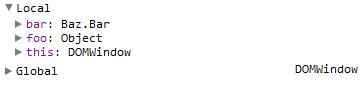
\includegraphics[width=0.47\textwidth,height=.15\textheight]{pic/chrome-objects.jpg}}
\hfil
\subfigure[Firebug]{\label{fig_object_first_case}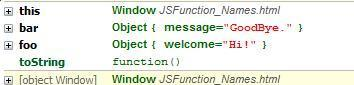
\includegraphics[width=.47\textwidth,height=.15\textheight]{pic/fbug-objects.jpg}}}
\caption{The screenshot of variables view of Google Chrome and Firebug JavaScript debuggers paused on a breakpoint at line 15 of the program shown in Figure~\ref{js-code}.}
\label{debuggers-objects}
\end{figure*}

To understand the consequences of anonymous functions on development tools we will focus on one example, the impact on debuggers.
Two main issues appear in debuggers due to the lack of function name. First, object constructor name, which can facilitate understanding the object value, is not available in the object summary. Second, the call-stack view is usually full of \textit{anonymous} functions and therefore much less informative. We discuss these issues in the next two subsections. 
 
\subsection{Missed Constructor Name in Object Summary}
JavaScript doesn't support classes, but objects can be created by constructors ({\small\texttt{new}} followed by a function call). A constructor is a regular JavaScript function. Once the {\small\texttt{new}} keyword is evaluated, an empty object, with the constructor prototype as its prototype, is created, then the new object is bound to {\small\texttt{this}} and the constructor is called. The role of constructor is to initialize the empty object. Unlike class-based object-oriented languages, the structure of object imposed by the constructor may change during the object's lifetime \cite{Richards}, the constructor can still be useful in classify the object.
Debuggers employ this fact and display the constructor name in the object summary to facilitate developer's understanding. 

Figure~\ref{js-code} shows an excerpt of a JavaScript program we use to illustrate this issue. We set a breakpoint on line 13 and examine the runtime elements at this breakpoint by two JavaScript debuggers, Google Chrome and Firebug (Figure~\ref{debuggers-objects}). Two objects assigned to variables {\small\texttt{foo}} and {\small\texttt{bar}} are constructed by two different constructors: {\small\texttt{FOO}} and {\small\texttt{BAR}}. However, Google Chrome debugger shows the general class of {\small\texttt{Object}} as the summary for both objects. The developer has to expand the object nodes to recognize their similarities and differences. Firebug classify objects in the same general class, but includes some of the object properties in the summary. These additional properties may hint the developer about the object structures. {\small\texttt{FOO}} and {\small\texttt{BAR}} definitions at lines 19 and 22 explain the debuggers' behavior; the function statements has no explicit name (identifier), therefore debuggers considered them as \textit{anonymous} functions.


\subsection{Anonymous Function Names in Call-stack View}
The second problem is the call-stack.
To illustrate this, we pause the program (Figure~\ref{js-code}) at line 15 by a breakpoint. Figure~\ref{debuggers-callstack} shows how the program call-stack is displayed in Google Chrome debugger and Firebug. The differences in the number of frames and line numbers between two call-stacks are due to dissimilar event handling implementations in the underlying platforms. Google chrome shows \textit{anonymous} as the name of all functions excepting the first one. Firebug performs better by guessing three function names but it still fails in one case. In these cases, the information provided by debugger is useless and the developer has to locate the function source to understand or recall the function behavior. 


\begin{figure*}[htp]
\centerline{
\subfigure[Google Chrome Debugger]{\label{fig_second_case}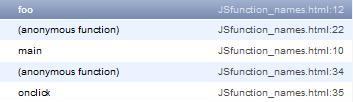
\includegraphics[width=0.47\textwidth,height=.13\textheight]{pic/chrome-callstack.jpg}}
\hfil
\subfigure[Firebug]{\label{fig_first_case}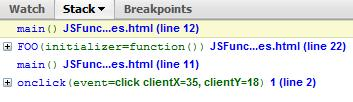
\includegraphics[width=.47\textwidth,height=.13\textheight]{pic/fbug-callstack.jpg}}}
\caption{The screenshot of call-stack view of Google Chrome and Firebug JavaScript debuggers paused on a breakpoint at line 15 of the program shown in Figure~\ref{js-code}.}
\label{debuggers-callstack}
\end{figure*}
 
%Two other pieces of information which are important at function calls are {\small\texttt{this}} and argument values. In JavaScript, {\small\texttt{this}} like arguments is not defined by lexical scopes but it is bound once the function is called. The {\small\texttt{this}} value is missed in both views. The {\small\texttt{arguments}} values is shown in Firebug, but it still suffers from the same issues as object summaries.

\section{Automated Function Naming}
The anonymous functions problem is discussed in several articles and forums on the Web \cite{DisplayName, Zaytsev}. Different solutions have been proposed and discussed by practitioners. A basic solution is a mechanism for naming functions by developers without affecting the variables in scopes. For example, a new property (e.g., \textit{displayName}) in the function object can be used for storing the function name, or the function name can be defined by an annotation. Although these solutions may help, they cause developers extra work, the displayName value can become out of sync with the meaning of the code over time,  the annotation may be incorrectly recognized in programs that use the same property name for another purpose, and maintenance of the debugger becomes more difficult once the call-stack names can be overridden by user code.

We instead propose an almost automated approach for naming all functions by analyzing the source code. Before getting into explaining the algorithm details we discuss the rationale behind some of decisions we made in this approach.

\subsection{What Should Be Named?}

Once a statement which defines a function is evaluated, a new {\small\texttt{Function}} 
object is created.  The definition may be evaluated multiple times, and depending on the times a function definition is evaluated, 
zero to many {\small\texttt{Function}} objects can be created from the same definition. 
Two function objects which are created from the same function body may have different object properties added at runtime. They also may have different enclosing scopes and therefore different behaviors.  Thus our first 
decision: do we try to name the {\small\texttt{Function}} objects or the source that defines them?

For the common use cases, the different {\small\texttt{Function}} objects are bound to one or more properties of objects. The  names of these properties inform the developer about the role of the function in the actions of the object.  To determine the actions of the functions in turn, the developer must read the function source (or perhaps its documentation). Our function names serve to recall or summarize that source or documentation for the developer. Therefore we seek to name the source, the content between the curly braces known as the {\textit{FunctionBody}} in the standard\cite{ECMA}.

After reflection the reader may be puzzled by the preceding claim. On the one hand we claim that the function object instance may be bound to properties in multiple objects and those property names are not helpful for naming. On the other hand we will shortly introduce an algorithm that uses a property name (in part) to name a {\textit{FunctionBody}}. Ultimately we are relying on a subtle characteristic of JavaScript programming: the first binding of a {\textit{Function}}  to an object property differs from all other bindings because it is located in text near the {\textit{FunctionBody}} and thus developers associate this first binding with the meaning of the {\textit{FunctionBody}}. 

\subsection{What Makes a Good Function Name?}
A function name is basically used to assist the developer to recall or understand the function behavior. For a developer who is already familiar with the function, it works more like an identifier. However, this identifier should be easily recognized by the developer. For example, a naive proposal for the function name is a combination of the function file name and its first line number. Although it may work as an identifier, but it does not assist the developer to recall or understand the function behavior.

 On the other hand, for a developer who does not know the function, a function name should explains the function behavior, or an abstraction of the function behavior, or why/where the function is used/defined (e.g., to create the object \textit{foo}). A function name must not be too long that can not be displayed or read by the developer. For example, the function body explains the function behavior well however it is not an appropriate function name.

\subsection{Context, Package and Function Names}
JavaScript does not support a standard packaging mechanism to be used for modular programming. Scripts are loaded from different files and executed within the same or different global objects. Developers usually use objects at the top level to encapsulate properties, objects and functions from a framework or library. The same mechanism is reused for defining subpackages. As the project size and the number of functions increases, the short function name will not be enough for recognizing the function. The developer also wants the class or the module contains the function. In addition to the package name, knowing the context (the enclosing function body) that contains the function can help in better understanding the function behavior.


\section{Building Up Intuition by Example}
We know that we face an ill-defined task: we are after all attempting to create short useful names for nameless functions. We have to create salient information from source code: we anticipate removing characters will be our biggest challenge.  To create an algorithm we decided to study the spectrum of examples from our 10 large collections of functions. We want to see what kinds of cases are important and what aspects of these cases help us identify functions.

For this purpose we created 12 categories of function body expressions shown in Table~\ref{table:function-types} and we categorized all of the nameless functions from the 10 libraries into one of 12 cases, giving the numerical results in Table~\ref{function-type-count}.  Then we examine each of these cases to think about how we want the functions named. We'll ignore nesting of function scopes in the analysis to avoid taking on too much at one time.
  
\begin{table}
\centering
\scalebox{0.8}{
\renewcommand\arraystretch{2.0}
\begin{tabular}{ | c | l | l | l | m{2.5cm} | l|}
  \hline
   & \multicolumn{4} {| c |}{Description} & \multicolumn{1} {| c |}{Code} \\ 
  \hline 
   
   1 &
   &  
   & \multicolumn{2}{|m{2.8cm}|}{
     \raggedright property of a new object in an object literal.}
   & \{ ..., foo: function()\{...\}, ...\}\\ %{\small\begin{verbatim}{ ..., foo: function(){...}, ...}\end{verbatim}} \\ %
   \cline{0-0}\cline{4-6}
	 
	 2 &
	 & \multirow{8}{*}{\hspace{.2cm}\begin{rotate}{90}is assigned to a(n)\end{rotate}}
	 & \multicolumn{2}{|m{2.8cm}|}{
	   new array index in an array literal.} 
   & [..., function()\{...\}, ...] \\ 
   \cline{0-0}\cline{4-6} 

   3 & \multirow{12}{*}{\hspace{.2cm}\begin{rotate}{90}The function object\end{rotate}} 
   & 
   &  
   & direct access by a property identifier.
   & bar\textsuperscript{*}.foo = function()\{...\}\\
   \cline{0-0}\cline{5-6} 

   4 & 
   & 
   & 
   & \raggedright hashmap access by a string. 
   & bar\textsuperscript{*}["foo"] = function()\{...\} \\
   \cline{0-0}\cline{5-6} 

   5 &
   & 
   & \multirow{4}{*}{\hspace{.2cm}\begin{rotate}{90}object property through\end{rotate}}
   & \raggedright hashmap access by a variable name.
   & bar\textsuperscript{*}[foo] = function()\{...\} \\
   \cline{0-0}\cline{5-6} 

   6 &
   & 
   & 
   & \raggedright hashmap access by a JavaScript expression.
   & bar\textsuperscript{*}[foo\textsuperscript{*}] = function()\{...\} \\
   \cline{0-0}\cline{4-6} 

   7 &
   &
   & \multicolumn{2}{|l|}{
      array index.}
   & foo\textsuperscript{*}[0] = function()\{...\} \\
   \cline{0-0}\cline{4-6} 

   8 &
   & 
   & \multicolumn{2}{|l|}{
      variable.}
   & foo = function()\{...\} \\
   \cline{0-0}\cline{3-6} 
   
   9 &
   & \multicolumn{3}{|m{3.8cm}|}{
     \raggedright is directly called.}
   & function()\{...\}() \\
   \cline{0-0}\cline{3-6} 

   10 &
   & \multicolumn{3}{|m{3.8cm}|}{
     \raggedright property is accessed.}
   & function()\{...\}.foo \\
   \cline{0-0}\cline{3-6} 

   11 &
   & \multicolumn{3}{|m{3.5cm}|}{
     \raggedright is returned from a function call.}
   & \{... return function()\{...\}\} \\
   \cline{0-0}\cline{3-6} 

   12 &
   & \multicolumn{3}{|m{3.5cm}|}{
     \raggedright is passed as an argument to a function.}
   & foo\textsuperscript{*}(..., function()\{\}, ...) \\
   \hline 

  \end{tabular}
    }
\caption{Different cases of anonymous function object creation and usage in JavaScript.  Identifiers with a star in the table can be expressions as well as simple identifiers; we explain how we reduce expressions to pseudo-identifier in ~\ref{sec:general-element-naming}.}
\label{table:function-types} 
\end{table}


\begin{table*}
\centering
\scalebox{0.8}{
  \begin{tabular}{ | l | l | l | l | l | l | l | l | l | l | l | l | l |}
  \hline
     & 1 & 2 & 3 & 4 & 5 & 6 & 7 & 8 & 9 & 10 & 11 & 12\\ 
  \hline 
   Closure       & 23(0.3\%)  & 0  & 8466(94\%) & 3  & 4  & 0  & 0 & 67(0.7\%) & 16(0.2\%) & 0  & 43(0.5\%) & 365(4\%)\\ 
  \hline 
   DOJO          & 9601(61\%) & 7  & 1765(11\%) & 21 & 24 & 2  & 1 & 1151(7\%) & 476(3\%) & 2  & 175(1\%) & 2641(17\%) \\ 
  \hline 
   ExtJS         & 30221(83\%) & 0  & 1476(4\%)  & 3  & 40 & 9  & 0 & 859(2\%) & 788(2\%) & 180  & 517(1\%) & 2439(7\%) \\ 
  \hline 
   Firebug       & 2296(76\%) & 0  & 539(18\%)  & 1  & 2  & 0  & 0 & 17(0.4\%) & 7(0.2\%) & 2  & 6(0.2\%) & 148(5\%) \\ 
  \hline 
   jQuery        & 233(58\%)  & 0  & 34(9\%)    & 0  & 10 & 2  & 0 & 24(6\%)  & 10(2\%)   & 0  & 0        & 86(21\%)  \\ 
  \hline 
   MochiKit      & 1080(59\%) & 10  & 385(21\%)  & 0  & 4  & 0  & 0 & 110(6\%) & 18(1\%)  & 0  & 41(2\%)  & 181(10\%) \\ 
  \hline 
   MooTools      & 339(55\%)  & 0  & 79(13\%)   & 0  & 4  & 3  & 0 & 53(9\%)  & 21(3\%)  & 20  & 14(2\%)  & 85(13\%) \\ 
  \hline 
   Prototype     & 265(60\%)  & 0  & 28(6\%)    & 0  & 0  & 1  & 0 & 25(6\%)  & 44(10\%) & 1  & 8(2\%)   & 70(16\%) \\ 
  \hline 
   Scriptaculous & 564(64\%)  & 0  & 75(8\%)    & 0  & 2  & 2  & 0 & 27(3\%)  & 45(5\%)  & 21  & 9(1\%)   & 139(15\%) \\ 
  \hline 
   YUI           & 14154(66\%) & 7  & 1721(8\%)  & 0  & 90 & 0  & 0 & 1181(6\%) & 172(1\%) & 0  & 95(0.5\%) & 4004(19\%)\\ 
  \hline 
   All           & 58776(65\%)& 24 & 14568(16\%)& 28 & 180& 19 & 1 & 3514(4\%)& 1597(2\%)& 226  & 908(1\%) & 10072(11\%) \\ 
  \hline 
  \end{tabular}
}
\caption{The number of nameless functions in each category defined in table~\ref{table:function-types}.}
\label{function-type-count} 
\end{table*} 


%     and extracting the initial name used for the function object after its creation. 
%In the third subsection we discuss qualities we expect from an automatically created function name.
 

\subsection{Case 1: Object Property Initializer}
 This case usually appears when developers try to group a set of functions in a new object. A common case is grouping a set of functions in the {\small\texttt{prototype}} property of the constructor. This structure resembles the class structure in traditional object-oriented languages. When a new object is created by the constructor, the new object also inherits all functions defined in the constructor's prototype. This structure is also used  when the owner object is a shared object with a set of utility functions.
 
 The majority of nameless functions (more than 65\%) in almost all studied projects (except Closure), are defined in object literals. This case seems particularly simple: the property name makes a good name for the function body. But what logic are we implicitly applying here? Our reasoning: the developer-invented property name has high information content, it is textually close to the function body, and the function object created by the function body initializes to the property. These observations guide us in more complex cases.
 
\subsection{Case 2: Entry in an Array Literal}
Contrary to the previous case the appearance of this case is very limited. It usually appears in initializations or when an array of functions are passed as an argument. Among all projects only two have instances of nameless functions defined in this way. For example array argument to \verb|Event._attach| in this example from YUI:
\begin{verbatim}
_attach: function (el, notifier, delegate) {
  if (Y.DOM.isWindow(el)) {
    return Event._attach([type, function (e) {
         notifier.fire(e);
    }, el]);
  }
}
\end{verbatim}
(The example is nested in more function definitions we do not show here). The developer will probably think of the array entry one item in a collection passed to \verb|Event._attach|. In general we shall want to name these kinds of functions by the destiny of the containing array.

\subsection{Case 3: Property Assignment With Property Identifier}
This case is the second most common case in the studied projects. Here, we can see why the Closure project is different from other projects in the first case. About 94\% of nameless functions in this project are defined in this way. It seems that the Closure developers follow an internal standard for function objects creation and usage.  

Following the model from Case 1, we expect a good name would combine the object name with the property identifier. The complication in this case comes from the object name: in general the object reference can be a computed expression. (This comment applies to all of the cases in table~\ref{table:function-types} marked with an asterisk on the expression identifier). Here is a simple example from the Closure project: 
\begin{verbatim}
  this.eventPool_.createObject = function() {
    return new goog.debug.Trace_.Event_();
  };
\end{verbatim}
 These expressions can be long and complex: to create a useful name we need to focus on developer-invented identifiers in the expression and work to keep the total number of characters small. For example, \verb|this.| add no information to the name since we can't know the value of \verb|this| while parsing. 

\subsection{Case 4: Property Assignment With  Property Name String}
In JavaScript, objects are like hashmaps and their properties can also be accessed by a string can be specified in the brackets after the object. Semantically this is the same as the previous case and we see few instances of this form for function object assignment. The string inside the brackets can be considered a property identifier for naming.

\subsection{Case 5: Property Assignment With  Property Name Variable}
Object member names can be variable references that get converted to strings at runtime: this is syntactically similar to Case 4, but we can't (usually) statically compute the string to use as a property identifier.
The usage of this case is also limited. This form usually appears when the same function body is assigned to different properties in a loop. 
For example see the inner function in Fig.~\ref{fig:jQueryEach}. The variable
 name in the cases we examined was generic name like {\small\texttt{o}} or {\small\texttt{item}}. Unlike the previous two cases, we
don't have a specific property name.  Nevertheless identifying the function body using the assignment target with the variable name as the property name follows the reasoning used for the simple cases.
\begin{figure*}[htp]
\begin{verbatim}
jQuery.each( "ajaxStart ajaxStop ajaxComplete ajaxError".split(" "), function( i, o ) {
    jQuery.fn[o] = function( f ) {
        return this.bind(o, f);
    };
});
\end{verbatim}
\caption{An example of functions passed as arguments to a function (row 11 in Table~\ref{table:function-types} and (the inner definition) an example of a 
function assigned to a hashmap using a variable name (row 5 in Table~\ref{table:function-types}. The function is from the jQuery library but simplified to fit on the page. }
\label{fig:jQueryEach}
\end{figure*}

\subsection{Case 6:  Property Assignment With  Property Name Expressions}
Object member names can be expressions that get converted to strings at runtime: this is more general than case 5. 
 A common case of expression in this case is a conditional expression, e.g., {\small\texttt{condition?"prop1":"prop2"}}, where the property that we assign the function to depends upon runtime values. Another kind of example of computed names comes from the Prototype project (refomatted to fit in the page):
\begin{verbatim}
  function define(D) {
    if (!element) element = getRootElement();
    property[D] = 'client' + D;
    viewport['get' + D] = function() { 
      return element[property[D]] 
    };
    return viewport['get' + D]();
  }
\end{verbatim}
The word \verb|get| is concatenated with the \verb|toString()| value of the argument \verb|D| at runtime to create the property name.  Unlike Case 5, the property name expression need not be a simple developer-invented identifier. In this example, \verb|viewport[getD]| could be a good name, but in general we will need to process the expression to balance length with information.

Notice that from the programming language point of view, Cases 3 through 6 are all special cases of Case 6. After all we are just selecting an object property in all of these cases.  But from a naming point of view these cases present different challenges and the more complex cases will make our necessary tradeoffs more costly.

\subsection{Case 7: Assignment to an Element of an Array}
We only observed one instance of this form in the studied projects. The numerical index should clearly be part of the name; the array name may be an expression that we have to analyze to create name.

\subsection{Case 8: Assignment to a Variable }
As the functions are immutable objects, it is very likely that a function object which is assigned to a variable, is used with the same variable name in the function scope
and its internal scopes. Although, there are cases that the variable name is temporary as the function is passed to another function or assigned to an object property, in most cases the variable name works will as the function name. 

\subsection{Case 9: Anonymous Functions Immediately Called}
Calling functions objects just after their creations is a common pattern in JavaScript. For example see the assignment to \verb|Y.ClassNameManager| in Fig.~\ref{fig:classnamemanager}; the function is called at the bottom of the example. 
\begin{figure}[htp]
\begin{verbatim}
Y.ClassNameManager = function () {

 var sPrefix    = CONFIG[CLASS_NAME_PREFIX],
   sDelimiter = CONFIG[CLASS_NAME_DELIMITER];

    return {
       getClassName: Y.cached(function () {
          var args = Y.Array(arguments);
          if (args[args.length-1] !== true) {
              args.unshift(sPrefix);
          } else {
              args.pop();
          }
          return args.join(sDelimiter);
      })
    };
}();
\end{verbatim}
\label{fig:classnamemanager}
\caption{An example the YUI project of function bodies from cases 9 (the outer function)  and 12  (the argument to Y.cached) from Table~\ref{table:function-types}  }
\end{figure}

If the called-function is assigned to a variable or object property, then we have a version of one of the other cases in Table~\ref{function-types}. The difference here is that we can tell from static analysis that the assignment will use the return value of the function, not the function object itself. But for naming purposes the key information will be the assignment target.

If the function call has no result, it means that the function performs one task (e.g., initialization of some values in the outer scope for later use). In this case we can't use the assignment target idea from Case 1, but source proximity and developer-invented names point to using interior identifiers in a name. To avoid confusing the developer by using the same name for the outer and interior functions, we will need some way to signify that the name we create this way is for an immediately called function.

\subsection{Case 10: Function Property is Accessed}
This case usually happens one of the predefined functions of function object (i.e., {\small\texttt{call, apply, bind}}) or an argument function to {\small\texttt{Function}} object prototype is called.

\subsection{Case 11:  Returned From a Function Call}

Although this category only includes 2\% of nameless function, proper naming of functions in this class is important. Many constructors are built using this form and therefore the names of these functions appear in object summaries.

\subsection{Case 12: Function Passed as an Argument}
Numbers in table~\ref{function-type-count} show that creating and passing functions as arguments is very common in JavaScript.
For example, see Fig.~\ref{fig:jQueryEach}. The calling function and the other arguments look helpful, to the extent that they have identifiers invented by the developer. As in the example we see that the calling function, \verb|jQuery.each()| can be generic so it provides less valuable information, but the arguments in that example are highly specific to the function body.  Fig.~\ref{fig:classnamemanager} shows different example, where the function called (\verb|Y.Cached()| seems much less important for naming the function than the property that we initialize with the result of calling the function.
This important case will stress any naming algorithm: we somehow have to summarize the function call -- which itself may be an expression -- and the other arguments -- any or all of which may be expressions. 

\subsection{Results of studying examples}
We reached two main conclusions from studying the way anonymous functions are used in the source of the 10 projects we examined. First, we want to try to find the name of the initializer or assignment target that will receive the function object created from a function body.  JavaScript programmers are creating anonymous functions but they are loading them into object references and the expressions that result in those references have informative identifiers inside. Second, these expressions that we focus on may often be simple identifiers, but if they don't we will need to analyze the source of these expressions to extract meaningful summaries. This summary has to balance information against length.

Overlaying our analysis above is hierarchy: any of the cases can be nested in function scopes. Obviously this hierarchy must be represented in our names. Algorithmically this is straight forward recursion. But from the name usability point of view, deep hierarchy means long names, exactly the problem we want to avoid. Fortunately developers are well trained in dealing with this kind of problem and we anticipate  that hierarchical names can be shown to users in progressive depth depending on the particular needs in the user interface.


%\subsection{Is it possible to automatically name functions?}
%\subsubsection{Static vs. Dynamic}
% Can we improve the names at runtime?
% function object path in dom model is good candidate for the name but only for persistent objects ?
%\subsubsection{Local vs. Global}
%the object bound to {\small\texttt{this}}-depending on the way the function is called-and passed arguments. The first two parameters can be almost known from the source code and are less dependent to the runtime while the last two parameters are usually not known until the function call at runtime. 
%\subsubsection{Is it possible to automatically name all functions?}
%\subsubsection{Other Challenges}%
% functions pass the name as string, different types of class definitions

\section{Static  Function Object Consumption}
Using our analysis we have created a preliminary automatic naming solution.  The three parts of our solution match three observations for our study. First we apply 
 \textit{(Static) Function Object Consumption}, which tracks the function object created from a function body to where the object is 'consumed', for example by assignment to or initialization of  an object property, variable reference, or function argument. The "static" qualifier just indicates that we will only use a parser.  Second, we reduce complex expressions to pseudo-identifiers focusing on developer-invented names.  Third we apply our approach hierarchically to  deal with nested function bodies.

We will describe the details in the next sections. In constructing names we realized one additional aspect: as we move from simple object property names to more complex examples, the path of the object consumption is an added bit of information helpful in naming. Thus we add some symbols to guide the developer to the function body in complex cases: this way the extra information does not take a lot of space and it can be ignored by developers who have not yet learned about its significance.


%To name a expression, we walk up the tree looking for the constructs in table 2. As we describe in section XX, for every matching construct we record identifiers or expressions to use in constructing a name. Then we assemble a name using the expression-reduction rules outlined in section YY and the context naming rules in section ZZ. The result is a summary that contains identifiers (i.e., variable and property names) and strings available in the source code plus some explanatory tokens. It compactly explains the function object creation, consumption and assignment. For the simple cases of function declaration, object property initialization, and variable initialization the algorithm gives the same results we described above.
 
%	We instead, to tackle the aforementioned issues caused due to the lack of function names, propose automated function naming by anlyzing the source code. Before getting into details of how the function name is constructed, we discuss the rationale behind some of decisions we made in this approach.
%  Developers usually understand and refer to function objects by aliases they use to access them. This fact particularly holds for permanent function objects such as classes and utility functions. However, functions with shorter lifetimes such as closures and callbacks are referred by their roles or purposes in the program. We employ these facts to construct an identifier for a function. We analyze the source code and build a summary that explains the function object creation, consumption and assignment.
%This summary which only contains identifiers (i.e., variable and property names) and strings available in the source code gives us the ingeredients for function identifier construction.
 %We analyze the source code to obtain the alias(es) that used for the function object or  is assigned to. If the list of aliases is not empty we select the most appropriate one based on some ranking rules as the function name. Otherwise, we try to build a name based on the aliases that the function object somehow affect on their values. If there is no such alias then the function object is consumed as an argument in a chain of function calls that does not return any value or as a simple closure. In the case of function calls chain we use the most nested called function name for constructing the identifier. In the case of simple closure, we employ the function(s) identifier inside the closure to construct the identifier. 
 %  On the other hand, it is very likely that the function object is assigned to this name in a place very close to the place the function object is created. Therefore, we analyze the code to find all names that the function object is assigned to them. For cases where the function object is not assigned to a variable or object property but is used to produce other values we keep track of the function effect on other identifiers.
      





%\subsection{Full Function Object Consumption Name}
\subsection{Consumption Summary Algorithm}
\label{sec:nodewalk}


We parse the JavaScript and search the resulting syntax tree for function body nodes. For each function body, we apply the algorithm outlined in Algorithm~\ref{alg1}. The basic idea (the \verb|while| loop) is to walk the syntax tree from the body up through parent nodes until we hit a node that is not a JavaScript expression. For each node we create an entry in a list and record in it information about the relationship between the node and its parent. We'll use this relationship information in Sec.~\ref{sec:concatenation}.Then for each node  we record developer-invented identifiers related to the destiny of the function object created from the body as outlined in  Table~\ref{table:node-types}. For the first and third rows of the table we record the information recursively; for the second row,  assignment node, we record the information after the loop terminates.   The algorithm ends when we reach a node which is an assignment or a statement which does not return any value (i.e., the node is not an expression).  The algorithm result is an \textit{object consumption summary}, a list of collected data at every visited parent node of the function body.

The algorithm uses three subroutines: \verb|getNextNode|,  \verb|nameExpression|, and \verb|argSummary|. The \verb|getNextNode| routine normally returns \verb|n.parent|, but we also use this point in the algorithm to handle an important special case, function bodies inside of \textit{immediate functions} typically used for modularity or scoping in JavaScript. We discuss this case in Sec.~\ref{sec:immediate}. The remaining two subroutines construct a pseudo-identifier from the expression as described in \ref{sec:general-element-naming}; they return their argument if it is simply an identifier.  


%\floatname{algorithm}{Procedure}b
\renewcommand{\algorithmicrequire}{\textbf{Input:}}
\renewcommand{\algorithmicensure}{\textbf{Output:}}

\begin{algorithm}                      % enter the algorithm environment
\caption{Compute Object Consumption Summary for Function Body Nodes}          % give the algorithm a caption
\label{alg1}                           % and a label for \ref{} commands later in the document
\begin{algorithmic}                    % enter the algorithmic environment
\REQUIRE Function Body Node $n$ in Abstract Syntax Tree
\ENSURE Object Consumption Summary 
\STATE $List$ $summary$ = $new$ $List$()


\WHILE {$n.parent$ is an expression}  
	\STATE $dataItem$ = $new$ $DataItem$()
    \IF {$n$ value is the same as $n.parent$ value}
    	 \STATE $dataItem.isTheSame$ = $true$
    \ELSIF {$n$ value is a property of $n.parent$ value}
    		\STATE $dataItem.isPartOf$ = $true$
    \ELSE	
	   		\STATE $dataItem.isContributesTo$ = $true$
    \ENDIF
    \IF {$n.parent$ is a function call and $n$ is an argument}
   	    \STATE $dataItem.isFunctionCall$ = $true$
   	    \STATE $dataItem.id$ = $nameExpression(n.parent)$
   	    \STATE $dataItem.hint$ = $argSummary(n.parent)$
   	\ELSIF {$n.parent$ is an object literal and $n$ is assigned to $foo$}
   	    \STATE $dataItem.isObjLiteral$ = $true$
   	    \STATE $dataItem.id$ = $foo$
    \ENDIF     
   \STATE $summary.add(dataItem)$
   \STATE $n$ = getNextNode($n$)
\ENDWHILE 
 
  \IF {$n.parent$ is an assignment} 
  	\STATE $dataItem$ = $new$ $DataItem$()
		\STATE $dataItem.isAssignment$ = $true$
    \STATE $dataItem.id$ = $nameExpression(n.parent)$
    \STATE $summary.add(dataItem)$
  \ENDIF	
  \RETURN $summary$
\end{algorithmic}
\end{algorithm}

\begin{table}
\centering
%\scalebox{0.8}{
\renewcommand\arraystretch{2.0}
\begin{tabular}{ | c | l | m{2.5cm} | l|}
  \hline
   & \multicolumn{2} {| c |}{Description} & \multicolumn{1} {| c |}{Code} \\ 
  \hline 

   1 & 
   & \raggedright an object literal.
   & \{ ..., foo: expr \}\\ 
   \cline{0-0}\cline{3-4}
	 
   2 & \multirow{4}{*}{\hspace{.2cm}\begin{rotate}{90}The parent node is\end{rotate}} 
   & 
     \raggedright a function call.
   & foo\textsuperscript{*}(..., expr, ...) \\
   \cline{0-0}\cline{3-4} 

   3 &
   & \raggedright an assignment.
   & foo\textsuperscript{*} = expr\\
   \cline{0-0}\cline{2-4} 

  \end{tabular}
%  }
\caption{Nodes produce identifiers in the function object consumption summary. Identifiers with a star in the table can be expressions as well as simple identifiers; we explain how we reduce expressions to pseudo-identifier in ~\ref{sec:general-element-naming}.}
\label{table:node-types} 
\end{table}

\subsection{Consumption by Immediate Functions}
\label{sec:immediate}
JavaScript developers use function scope to dynamically create functions with shared but private state. In this pattern, an enclosing function contains a number of function and object definitions and it is called immediately after it is defined. We call these functions \textit{immediate functions}.  For an example, see line 10 of the Listing~\ref{js-code} which is enclosed in the function on line 9. If the developer returns a function from this outer, immediate function we want to follow the returned object to where it is consumed. 

To keep our core algorithm simple we handle these returns from immediate functions as a special case. At the end of each loop in Algorithm~\ref{alg1} at the point marked \verb|getNextNode()| we check to see if our parent is a \verb|return| node.  If not we return the parent node and the loop continues. If we have a \verb|return| node, we look to the parent of the \verb|return| node to see if it is a call (either directly with \verb|()| or via \verb|apply()| or \verb|call()|. If so, we know we are returning a function object from an immediate function.  We return the parent of the immediate function, effectively skipping the intermediate nodes so that the name will reflect the consumption of the return value into the destination of the immediate function.

\subsection{Expression Reductions}
\label{sec:general-element-naming}

In simple cases the syntax tree node will have an identifier we can use as part of our name. In more complex cases an expression will written in place of an identifier. We reduce these expressions to pseudo-identifiers (i.e. not necessarily a valid JavaScript identifier) that resembles the expression. This work is done during the Object Consumption Summary algorithm in the functions described here:
\paragraph{Identifiers for Function Arguments} Search for all string nodes in other arguments and concatenated them by ``-'', dropping  characters over 10.  
 (This work is on in Algorithm~\ref{alg1} in \verb|argSummary|).
\paragraph{Identifiers for Assignments and Function calls} This function gets called for nodes resulting from the first 6 rows of Table~\ref{table:function-types}. The expressions here will evaluate to a writable address, so we want to extract the most specific developer-invented identifiers from the expression. Thus we apply the rules from Table~\ref{expression-reduction}, which starts from the right hand side of the expression;  we skip any JavaScript keywords like \texttt{this} or \texttt{prototype}. If we encounter any pattern which does not match, for example a function call, we stop.   (This work is on in Algorithm~\ref{alg1} in \verb|nameExpressions|.)

Obviously these rules are heuristic and can be improved through experience and interaction with developers. We are attempting to balance information content with length. Large complex expressions will give pseudo-identifiers which are complex, but with some identifiable parts.

\begin{table}
\centering
\scalebox{0.9}{
  \begin{tabular}{ | l | l | l |}
  \hline
   Description &Pattern &  Name \\ 
  \hline 
   Primitive & value & value.toString() \\ 
  \hline 
   Variable & id & id \\ 
  \hline 
   GetProp & e.id & Name(e).id \\ 
  \hline 
   GetElem & e1[e2] & Name(e1)+``['+'Name(e2)+``]'' \\ 
  \hline 
   Add & e1 op e2 & Name(e1)+op+Name(e2) \\ 
  \hline 
   Condition & cond?e1:e2 & Name(e1)+":"+Name(e2) \\ 
  \hline 
  \end{tabular}
  }
\caption{JavaScript Expression Reduction to a Name. Expressions which match an entry in the pattern column are converted as shown in the Name column. Here \texttt{e} indicates an expression, \texttt{id} indicates an identifier, \texttt{+} means string concatenation and \texttt{Name()} means we apply the pattern matching recursively.}
\label{expression-reduction} 
\end{table}    

\subsection{Conversion to an Name}
\label{sec:concatenation}
At this stage of the algorithm we have a list of identifiers with attributes which we want to concatenate to create a name. 

First we drop function-call identifiers if we have anything else to use for a name. The function-call identifiers typically tell us about a transformation of the function body before it is assigned to an object property or variable. The transformation may be used many places in the code, while the assignment target is typically an identifier defined by the developer.  See for example function on line 14 and the function call on line 13 in the Listing~\ref{js-code}. Specifically we drop identifiers from row 2 of table~\ref{table:node-types} in any case where have identifiers from rows 1 or 3.  The outer function in Fig.~\ref{fig:jQueryEach} illustrates the opposite case, where we don't drop function-call identifier. 
 
Second we concatenate the identifiers with a symbol between each parent and child showing the relationship.  As shown in Algorithm~\ref{alg1},  
if the parent expression is an array or object literal then the identifier will be marked  as \textit{isPartOf} and we insert a dot character. If the identifier was marked as  \textit{isContributesTo} we insert a left angle bracket. An identifier marked \textit{isSameAs} is skipped over because we already have identifier information for it. Because some entries on the object consumption list are empty strings we may have duplicate symbols. Any duplicates are replaced a single symbol. The result contains identifiers (i.e., variable and property names) and strings available in the source code plus some explanatory tokens. It compactly explains the function object creation, consumption and assignment.
 

The particular symbols we use may be refined with more experience in how developers respond to them. Our intuition is that these extra symbols need to be visually compact because their purpose is to adjust the developers expectation for the identifier. For example, the function on line 9 of Fig.~\ref{fig:js-code} is named \texttt{main<} but the developer may only key on the word \texttt{main} to recall the function body. 

The name is built by the above process does not contain any information about enclosing scopes. We call it \textit{local name}. We get the function \textit{full name} by adding the enclosing function full-name with a slash before the local-name, recursing through enclosing scopes. This full-name is our function body name.


%\section{Improved by Runtime Data}
%\subsection{Naming Functions in Call Stack}


\subsection{Example}
  
To further explain our approach we now apply it to the JavaScript code presented in Figure~\ref{js-code}. We can recognize seven function bodies in the code, none of them has a name. 

The first function on line 9 is called just after its creation (see line 18) and the return sets the {\small\texttt{main}} value. We can explain the function object consumption after its creation in two steps. First the parent node is a function call (row 2 in Table~\ref{table:node-types}. 2) the result is assigned to {\small\texttt{main}}. This differs from the simple variable assignment case: the value of {\small\texttt{main}} is not a function object but rather the return value of a function object.   We summarize this by saying that the result object is produced by the function object or the function object contributed to the {\small\texttt{main}} value and we write it {\small\texttt{main<}}, where the symbol {\small\texttt{<}} indicates "contributes to".

The function in line 10 is returned just after its creation. This function is located inside a closure function (i.e., a function which is called directly after its creation). This structure lets us to continue the static function object consumption analysis by assigning the return expression (the function body in line 10) to the alias set by the closure call result ({\small\texttt{main}}). The summary of the function object consumption will be: 1) the function object is returned , 2) the function object is assigned to {\small\texttt{main}}. As the function object is directly assigned to this variable we name the function {\small\texttt{main}}.

The third function, line 14, is passed to a function {\small\texttt{op}} on line 13, within the body of the function we named {\small\texttt{main}} . Here 1) the function object is passed as an argument to function {\small\texttt{op}}, 2) The call result is assigned to {\small\texttt{result}}. If we simply put the identifiers in the summary together we get {\small\texttt{main/result<op()}}. The first part before slash  shows the context name (the enclosing function name) for this function.  However, the function names (here {\small\texttt{op()}}) usually give an indirect information (e.g., role) about the function object. Therefore, as we explain in 4.5, we ignore them if other kind of identifiers (e.g., variable and property name) are available in the summary. After dropping {\small\texttt{op}}, we will have {\small\texttt{main/result<}}. Eliding identifiers is important to avoid creating long, unwieldy names.

The next two functions, {\small\texttt{FOO}} on line 19 and {\small\texttt{BAR}} on line 22 are simple examples of case 6.  The last two functions defined in lines 25 and 27, similar to functions in lines 9 and 10, are named {\small\texttt{op<}} and {\small\texttt{op}} respectively. 



\begin{table*}
\centering
\scalebox{0.8}{
  \begin{tabular}{ | l | l | l | l | l | l | l | l | l | l |}
  \hline
   Project       & Anonymous &  FBUG NoName   & NoName   & NoShortName &    = FBUG Name     & \texttildelow FBUG Name & Duplicates  & Avgerage      & Longest  \\ 
  \hline 
   Closure       & 8987      &   312(3\%)     & 10       &  51         &    66(0.7\%)         &    8462(94\%)         & 113(1\%)    & 33/35         & 76/101 \\ 
  \hline 
   DoJo          & 15866     &   3362(2\%)    & 390      &  528        &    3067(19\%)        &    9115(57\%)         & 2677(17\%)  & 35/36         & 81/162 \\ 
  \hline 
   ExtJS         & 36533     &   1543(4\%)    & 231      &  631        &    4007(11\%)        &    13572(37\%         & 2573(7\%)   & 22/25         & 65/91  \\ 
  \hline 
   Firebug       & 3018      &   167(5\%)     & 10       &  14         &    397(13\%)         &    2442(80\%)         & 2976(1\%)   & 27/36         & 70/140 \\ 
  \hline 
   jQuery        & 399       &   95(24\%)     & 8        &  9          &    151(38\%)         &    131(33\%)          & 64(16\%)    & 14/18         & 50/65  \\ 
  \hline 
   MochiKit      & 1829      &   202(11\%)    & 16       &  59         &    779(43\%)         &    789(43\%)          & 207(11\%)   & 17/22         & 49/80   \\ 
  \hline 
   MooTools      & 618       &   121(19\%)    & 18       &  30         &    266(43\%)         &    180(29\%)          & 156(25\%)   & 12/14         & 36/73   \\ 
  \hline 
   Prototype     & 442       &   125(28\%)    & 19       &  24         &    38(8\%)           &    272(62\%)          & 89(20\%)    & 23/25         & 55/88    \\ 
  \hline  
   Scriptaculous & 884       &   195(22\%)    & 19       &  25         &    79(8\%)           &    573(65\%)          & 105(12\%)   & 22/27         & 55/132   \\ 
  \hline    
   YUI           & 21424     &   3317(15\%)   & 15       &  212        &    4846(23\%)        &    6962(33\%)         & 2220(10\%)  & 16/37         & 114/145  \\ 
  \hline 
   All           & 90000     &   9439(10\%)   & 736(1\%) &  1583(2\%)  &    13696(15\%)       &    42498(47\%)        & 8264(9\%)   &                &          \\ 
  \hline       
  \end{tabular}
  }
 \label{evaluation} 
\caption{Results of Function Object Consumption. The rows are the projects listed in Appendix 1. First column in  contains the number of anonymous functions in each project. The second column shows the number of functions Firebug could not name. The third column contains the number of functions nameless after applying the static Function Object Consumption (FOC) algorithm;  and the fourth column is the number with only a name for enclosing scopes. The fifth column give the number of times a FOC function name appears twice in a file and sixth and seventh columns give the average and longest name character counts respectively. The last columns have two entries divided by a slash, the first is the local name and the second is the full name.} 
\end{table*}    

\section{Evaluation}
The purpose of our evaluation is to answer the following questions: 1) How effective is the approach in naming anonymous functions? 2) How the algorithm  improves the current approaches used in available debuggers for inferring anonymous function names? 3) Are the proposed names are unique to be used as identifiers or conversely what portion of proposed names are duplicated? 4) Are the proposed names appropriate for user interface presentation? 

In Table~\ref{evaluation} We compared our results to Firebug's naming output for each of the 10 projects used previously and listed in Appendix 1. Firebug does not use a parser for naming functions. It instead employs a number of regular expressions and apply them on a few lines around the function definition to obtain a name  (a function called {\small \texttt{guessFunctionName()}}). Although this approach is not reliable and may provide wrong names for some functions, it infers acceptable names in many simple cases. About 10 percent of anonymous functions still remained nameless in Firebug (in addition, some named functions may be quite incorrect because of the simple algorithm).The numbers show that the algorithm names more than 99 percent of the anonymous functions.


The duplicates column show the number of duplicated function names. About 9 percent of inferred names used for more than one function in a file. The main source of duplicated names are test cases particularly in DOJO, ExtJS and YUI. 
%the other sources :1) function calls with no hint  2) conditional functions (e.g., based on browser)

The last two columns show the average and longest function name lengths (in characters) for both short and full names. The average length is at most 37 characters. The longest  names are typically long because of a long local name.  

%\subsection{Produced Names Characteristics}
%\subsection{Developers' vs. Automated Names}
%\subsection{Compared to Firebug {\large \texttt{guessFunctionName()}}}

%\subsection{Manual Check}
%namespaces in JS:http://javascriptweblog.wordpress.com/2010/12/07/namespacing-in-javascript/
%commonjs requriejs, ...
%the function name not very long like google chrome  xxxx.yyy.zzz

%Firebug uses a utility function called {\small \texttt{guessFunctionName()}} to name nameless functions.This algorithm used in the function searches lines around the line the function definition line for specific patterns by regular expressions. The  first string matches one of the patterns becomes the name of the function. We compared the results of our algorithm to Firebug's in table~\ref{firebug}.
%The first column shows, how many functions get similar names by both algorithm. In average, for 60\% of functions both algorithms produce the same names. Firebug is not able to name about 15\% of functions. In 35\% of functions the results are different. In most cases, the proposed name by Firebug is the name of another function and is wrong. 
   

\section{Discussion}
Overall the Function-Object Consumption approach dramatically improves reduces the number of functions that a development tool cannot name for a developer.  By looking at the examples and comparing the algorithms, the names selected by FOC will be the same as the one's selected by  Firebug's {\small \texttt{guessFunctionName()}} when that function gives reasonable results. In other cases FOC will give a more useful name including many cases where the current Firebug approach fails. 

There is room for improvements. The heuristic elements of the naming solution need to be tuned based on more experience.  Given that our goals trade precision for rapid recognition, our names are not unique. We also leave some cases anonymous which need further investigation. 


\subsection{Similar Function Names in a File}
In some cases function bodies are named with the same names in a file. It can happen in different situations. One of the common cases is the two different function bodies may assign to a property based on a condition (e.g., the browser). For these cases we add a dollar sign and an index to the similar function names. For example, if there are two function bodies with names {\small\texttt{myFunction}}, the functions are named as {\small\texttt{myFunction\$0}} and {\small\texttt{myFunction\$1}}. 

\subsection{Namer Functions}
Many JavaScript projects have one or a few functions which are used for defining classes or registering function objects. These functions usually receive a string as the class name or function name. The number of namer functions is usually very limited for a specific project and can be provided to debugger by the developer. A namer function works like an assignment in the summary.  

% to register a function with a name
% to wrap the function
% as a callback


\subsection{Functions created by {\large \texttt{eval()}}}
The function bodies in {\small\texttt{eval}} statements can be named similar to other objects as the source code is available. However, eval scripts have no file name and therefore, it causes issues for assigning appropriate packages name to these functions. 

\subsection{ {\texttt .displayName} }
The ultimate fallback for function names is to allow the developer to specify them manually. For application developers this is tedious path, but for library developers the cost may be justified by the many potential developers who will see the custom name.

%\subsection{Limitations}
%some long names
%"this" in names

% open problems: naming scripts loaded and evaluated by eval,
\section{Related Work}
% Andrew Ko paper about errors by names
% ecoop 2009 paper
% typing system papers

%JavaScript, unlike many traditional object oriented languages such as Java and C\#, does not have classes, and does not encourage encapsulation or even structured programming. JavaScript is a weakly typed language with no type declarations and only run-time checking of calls and field accesses \cite{Richards}. As a direct consequence, the JavaScript code contains less explanatory data about the program elements and their relations. For example, the value of a variable can be a primitive value, an object with any structure or even a function. One call-site may invoke different function bodies with various number of arities that none of them can be understood from the code. Therefore, the lack of descriptive data in JavaScript code is the most fundamental issue in enhancing JavaScript tool support.


Catching errors early (i.e., before or at the compilation time) is an important feature for development environments. It can save developers' time, prevent bugs and improve the program quality. However, many errors can not be recognized without a strong typing system. To attack this issue a few static typing systems have been proposed for JavaScript \cite{Anderson, Anderson2, Heidegger, Thiemann}. These approaches discover the type of values and object structures for a variable by statically analyzing the source code and possible program control flows lead to the variable assignment. The discovered facts about variable types are not only useful for catching errors but to provide modern editing features such as auto-complete and refactoring in development environments. Moreover, the inferred data can help in code comprehension if they are properly presented. Nevertheless, none of the mentioned approaches provided effective means for sharing this information with the developer. This leads us to another hidden issue for improving JavaScript development tools; Due to highly dynamism in JavaScript many elements are remained nameless. Therefore there is no common language between the tool and developer for referring to elements.

%Developers usually understand JavaScript code by examining the running program in debuggers. At runtime, concrete values are available and the developer can directly check and understand object structures and control flows. Understanding a concrete value, particularly for non-primitive values such as objects and functions, is not always straightforward. To facilitate understanding these complex values in the first place, debuggers show a summary of these objects. For example, in the case of user-defined objects, the name of object's constructor in the object summary can be very helpful. It works like a class name in class-based languages and suggests the object structure.

\section{Conclusion}
Our contributions in this paper include an empirical study of the extent of anonymous functions in JavaScript libraries, categorization of those functions to understand the potential for automatic naming, an practical algorithm based on the empirical study, and its evaluation.   We believe our results can be applied directly in existing JavaScript development tools to give immediate benefit to developers and they provide a basis for future improvements.



\appendix
\section{JavaScript Projects Analyzed for Function Names}
\begin{description}
\item[Closure] Google Web Library, ...
\item[Dojo] JavaScript Toolkit
\item[ExtJS] JavaScript Framework
\item[Firebug] Web Page Debugger, http://code.google.com/p/fbug/, version 1.7??
\item[jQuery]
\item[MochiKit]
\item[MooTools]
\item[Prototype]
\item[Scriptaculous]
\item[YUI]
\end{description}



%\acks

%Acknowledgments, if needed.

% We recommend abbrvnat bibliography style.

%\bibliographystyle{abbrvnat}

% The bibliography should be embedded for final submission.

%\begin{thebibliography}{10}

\begin{thebibliography}{}
\softraggedright

%\bibitem[Smith et~al.(2009)Smith, Jones]{smith02}
%P. Q. Smith, and X. Y. Jones. ...reference text...

\bibitem{Anderson}
C. Anderson, P. Giannini, and S. Drossopoulou. \newblock Towards Type Inference for JavaScript.
\newblock In \emph{Proceedings of the 19th European conference on Object-Oriented Programming(ECOOP)},
July, 2005.

\bibitem{Anderson2}
C. Anderson and P. Giannini. \newblock Type checking for javascript.
\newblock \emph{Electr. Notes Theor. Comput. Sci.}, 138(2), 2005. 

\bibitem{CJS}
Common JS.
\newblock http://www.commonjs.org/

\bibitem{DisplayName}
Add prettyName/displayName support to Profiler output and Stacks.
\newblock \emph{Firebug Bug Repository},
\newblock http://code.google.com/p/fbug/issues/detail?id=1811

\bibitem{ECMA}
ECMA International.
\newblock \emph{ECMA-262: ECMAScript Language Specification},
ECMA (European Association for Standardizing Information
and Communication Systems), Geneva, Switzerland, third edition,
December 1999. 

\bibitem{FAO}
Firefox Add-ons.
\newblock https://addons.mozilla.org/en-US/developers/docs/gett ing-started.

\bibitem{GCE}
Google Chrome Extensions.
\newblock http://code.google.com/chrome/extensions.

\bibitem{Heidegger}
P. Heidegger and P. Thiemann.\newblock Recency types for dynamically-typed, object-based languages.
\newblock In \emph{Proceedings of Foundations of Object Oriented Languages (FOOL)},
2009.

\bibitem{Ingalls}
D. Ingalls, K. Palacz, S. Uhler and A. Taivalsaari.\newblock The lively kernel a self-supporting system on
a web page.
\newblock In \emph{Self-Sustaining Systems},
2008.

\bibitem{JSOffice}
JScript development in Microsoft Office 11.
\newblock http://msdn.microsoft.com/ en-us/library/aa202668(office.11).aspx

\bibitem{JSOffice2}
JavaScript development in OpenOffice.
\newblock http://framework.openoffice.org/ scripting/release-0.2/javascript-devguide.html

\bibitem{Richards}
G. Richards, S. Lebresne, B. Burg and J. Vitek.\newblock An analysis of the dynamic behavior of JavaScript programs.
\newblock In \emph{Proceedings of the 2010 ACM SIGPLAN conference on Programming language design and implementation(PLDI)},
June, 2010.

\bibitem{SSJSR}
Server-Side JavaScript Reference v1.2.
\newblock http://research.nihonsoft.org/ javascript/ServerReferenceJS12.

\bibitem{Thiemann}
P. Thiemann.\newblock Towards a type system for analyzing JavaScript programs.
\newblock In \emph{Proceedings of European Symposium on Programming (ESOP)},
2005.

\bibitem{Zaytsev}
J. Zaytsev.\newblock Named function expressions demystified.
\newblock http://kangax.github.com/nfe,
June, 2010.


\end{thebibliography}




\end{document}
